Besides of this report, my project --that is meant to practically demonstrate the feasibility of the architecture in figure~\ref{img:architecture}-- is composed of three different types of applications. Two JavaScript applications, the \emph{kernel} and the \emph{consumer application} that together form the visEngine and, a \emph{sample application}, a collection of vism and vis files that are meant to be used by this very same engine in order to render different usable interfaces. It is easiest to take the sample application as a starting point and from there, progressively explore the details of how the visEngine actually generates the visible result. The sample application contains the minimal set of interfaces necessary to engage a discussion about the most critical aspects of the system.

\begin{figure}
    \centering
    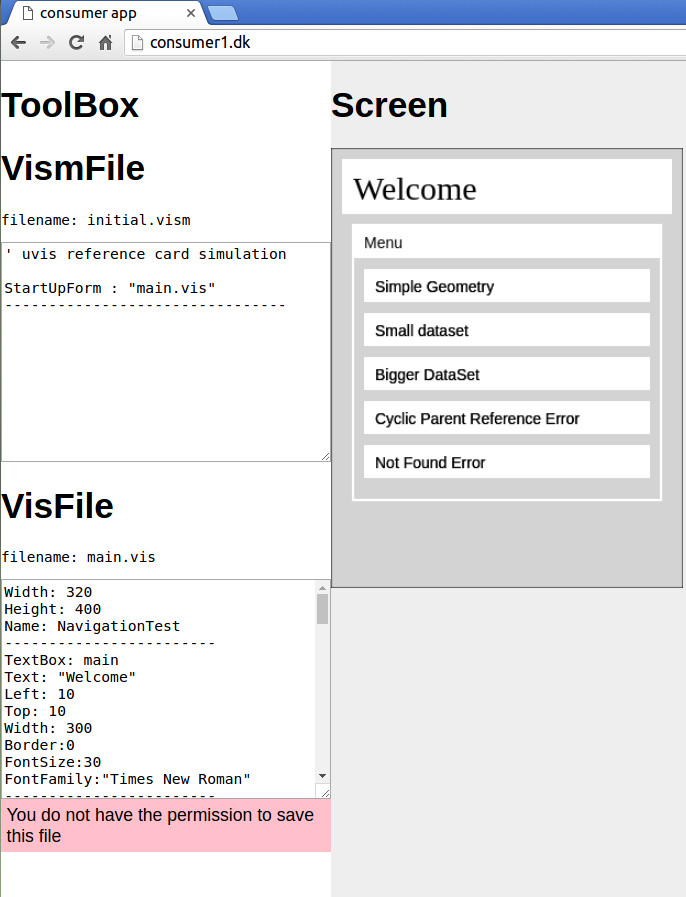
\includegraphics[width=0.9\textwidth]{images/home.jpg}
    \caption{Sample application home page}
    \label{img:home}
\end{figure}

It is accessed by the end-user through the browser by navigating to the url address that is bound to the domain application. 
\todo[inline]{give the address to the application here} When accessed, the user finds himself in front of an interface that shows a toolbox and a screen similar to what is shown in figure~\ref{img:home}.

\paragraph{The toolbox} shows a vism file and a vis file. It's current implementation has nothing to do with the toolbox that appears in the real system. In our case it is oversimplified. It's only purpose is to help the reader understand the connection between the description files presented withing it and the resulting screen on it's right-hand side. It actually also works for edit the vis files if setting the kernel to the correct mode. A complete toolbox would allow to drag and drop the components etc. The current implementation is good enough in order to show the feasibility of the desired architecture.

\paragraph{The screen} shows the rendered graphical user interface of what is described in the vis file. From the Toolbox the connection between the vism file, the vis file and the final screen appears at first glance. Here, the engine first opened the vism file based on the given url address, it retrieved the name of the vis file to open on startup, downloaded it and generated the screen that (hopefully) most users will understand. The vis file describes how the screen is built. A welcoming title is displayed and under it, multiple navigable links help the user to orient himself throughout the application.

\begin{figure}
    \centering
    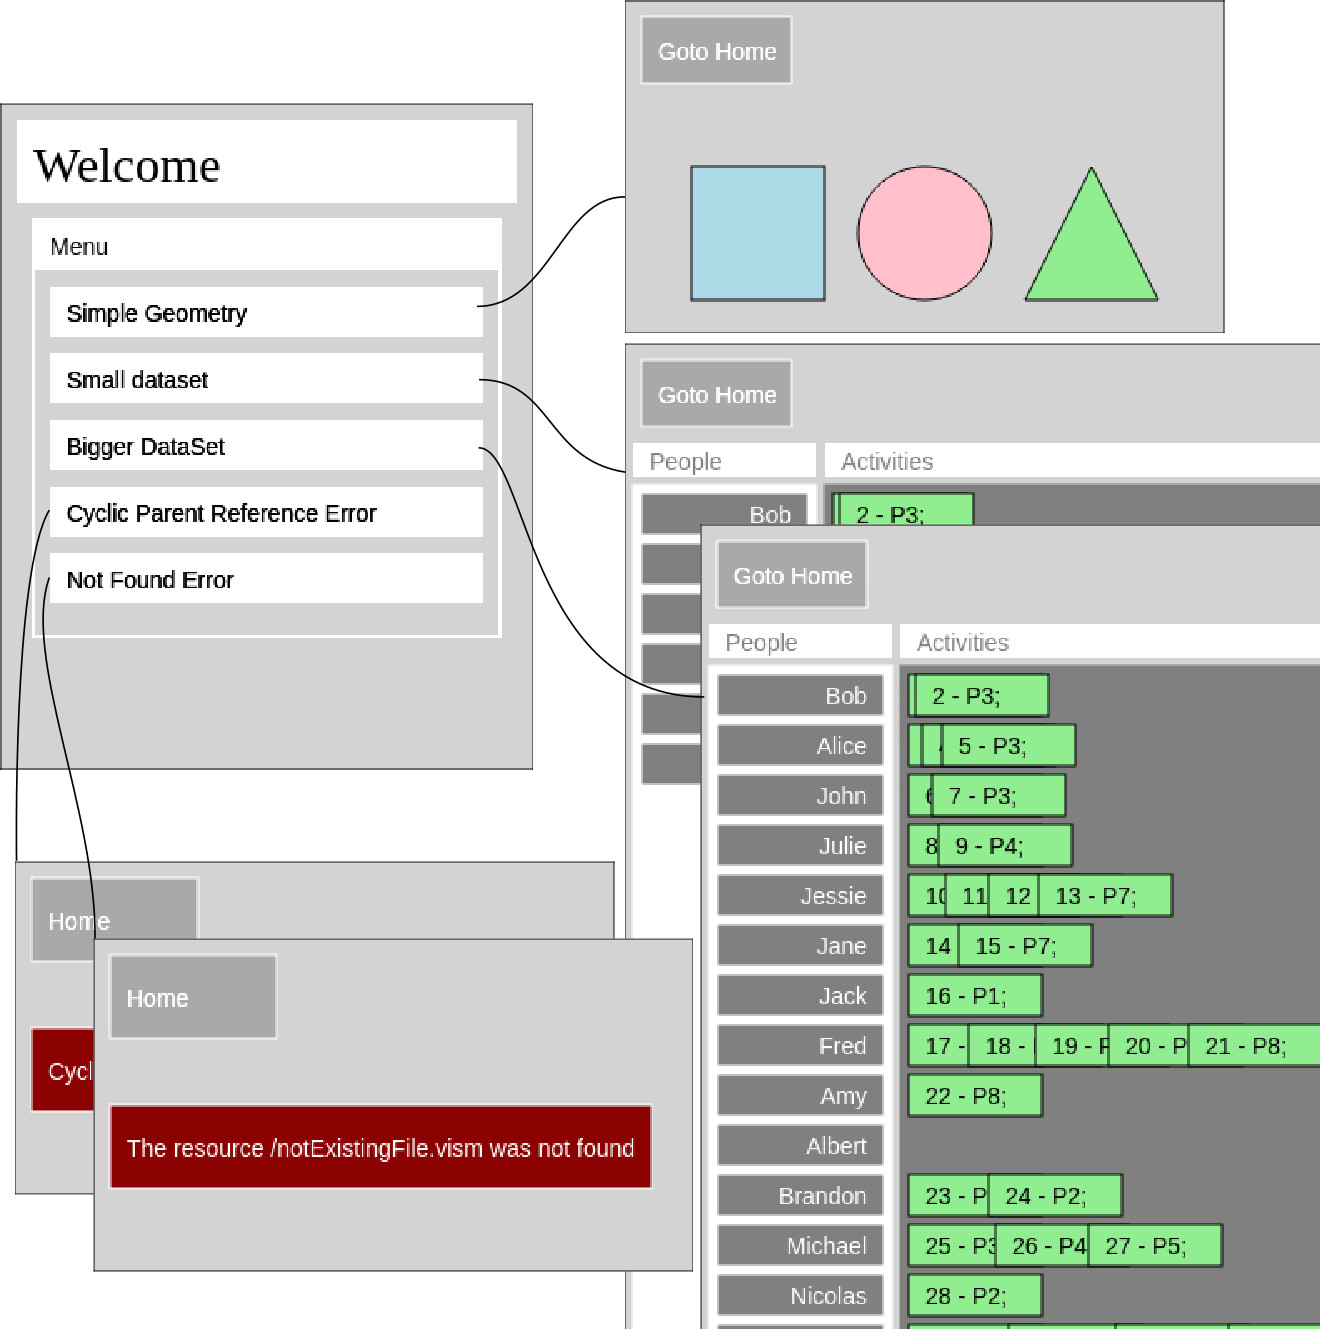
\includegraphics[width=0.9\textwidth]{images/screens.jpg}
    \caption{Sample application screen diagram}
    \label{img:screens}
\end{figure}

Figure~\ref{img:screens} shows a diagram over the different screens that are part of the sample application. On the upper-left corner of all screens that are related to the menu, a button takes the user back to that initial page from where he can easily navigate to the other screens.

The menu itself represents an interface on the background of which I will discuss how the kernel and the consumer application communicates together and how the interaction between the end-user and the components is made possible.

The first entry in the menu, if clicked, brings to an interface that shows a screen made of simple geometrical figures. This screen is the result of a vis file where components that are registered externally to the kernel, by the developer, have been addressed by the designer. To understand how external components can be registered into the kernel it also requires to understand how built-in components are registered.

The second and third menu entry links to screens that trigger calls to the most critical parts of the kernel and to what makes VisTool a very unique data-visualisation tool. Further they show how the local-developer can easily switch between different databases using different vism files to test different data-scenarios with the same interface.

The forth link points to an interface that illustrates how the system catches a cyclic parent reference. As I have described above, if not properly caught, this would cause the program to run into an infinite loop.

The last link leads to a screen showing another type of error that occurs if an user tries to access a vism file that does not exist.